\documentclass[10pt,letterpaper]{article}
\usepackage[latin1]{inputenc}
\usepackage{amsmath}
\usepackage{amsfonts}
\usepackage{amssymb}
\usepackage{graphicx}
\usepackage[left=1.00in, right=1.00in, top=1.00in, bottom=1.00in]{geometry}
\usepackage{subfigure}
\begin{document}


\section{Dataset description}
We will primarily be analyzing the CropScape\footnote{https://nassgeodata.gmu.edu/CropScape/} data from, United States Department of Agriculture
National Agricultural Statistics Service From 2008 - 2016. This is mainly, geo-referenced, raster image data created annually for the continental United States using moderate resolution satellite imagery and extensive agricultural ground truth. Each pixel in this raster image data identifies a geographical area. The data has information like crop-specific planting frequency per pixel, which is based on land cover information between the years 2008 and 2016 . The data identifies the spatial distribution of multiple crops across the US through the last nine years. There are currently four individual crops for which complete data is available, these are: corn, cotton, soybeans, and wheat. In our study we will be focusing on the distribution of corn at the level of counties and use the Cropscape data as our ground truth. Below is the land cover satellite image and the corresponding corn planting data for Montgomery county in 2016. 

\begin{figure}[ht]
\hfill
\subfigure{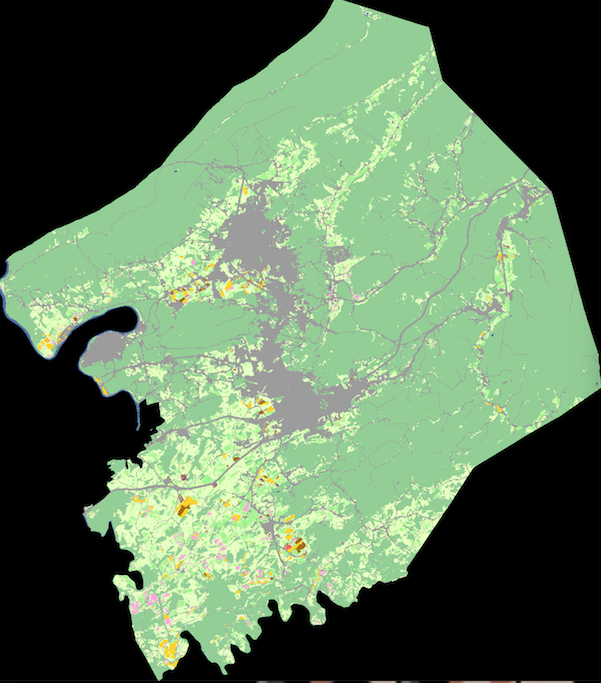
\includegraphics[width=5cm]{satellite.png}}
\hfill
\subfigure{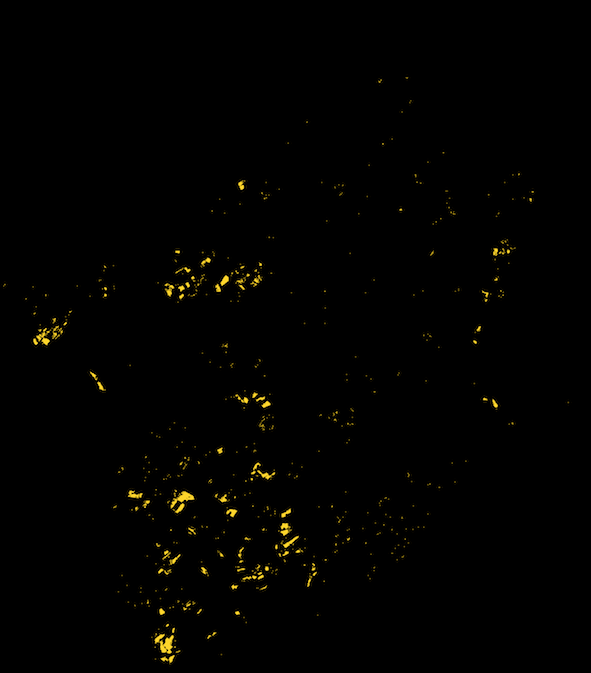
\includegraphics[width=5cm]{corn.png}}
\hfill \hfill
\caption{Sample satellite and corn cultivation image for Montgomery county}
\end{figure}

\noindent
In the image on the right hand side, each of the yellow pixels represent that corn has been planted on the corresponding geographic locations, for those pixels in 2016. 

\section{Questions to be answered using data analysis}


We will be answering the following three questions using our analysis:

\begin{enumerate}
	\item Given the satellite image of a county, can we predict how many pixels (acres of land) are present in that county on which corn is being grown?
	\item Can we accurately predict the pixel-wise distribution of crops (specifically corn) in a particular geographic area (county) of the United States?
	\item Can we augment the raster image data with additional freely available data for each pixel like: elevation (using something Google maps API), latitude, longitude, average annual temperature, average annual precipitation (rain and snow), distance from the sea, distance from the nearest water source, etc.? How does this impact the prediction accuracies?
\end{enumerate}

\noindent
This is not an exhaustive list, we might explore more questions if time permits. We would work on these questions in sequence, i.e. we will start with the first two questions and then work on the third question. 

\section{Data analytics techniques that will be used in the analysis}

We will primarily be employing the following three techniques, however we might add others to this list if they seem to be useful:

\begin{enumerate}
	\item Decision trees
	\item Support vector machine
	\item Ensemble methods (random forests, boosting, bagging, etc.)
	\item Neural networks (deep learning)
\end{enumerate}

\noindent
The first two are proven techniques for exploratory data analytics and these will help us establish a baseline for evaluation. Ensemble methods generally outperform individual classifiers, so these might help us improve the baseline obtained from the first two techniques. Deep learning has been successfully used in many computer vision applications in the past, and we feel it will be an interesting approach for our problems, as we will be dealing with raster image data.

\section{Evaluation techniques that will be used}

We will be using k-fold cross validation, and will evaluate our approach using the following evaluation metrics:
\begin{enumerate}
	\item ROC curves
	\item Accuracy
	\item F-measure
\end{enumerate}

\section{References to existing and related work}

The following two papers are based on Cropland data, we will be using these for our first question and will be extending these for the last two questions:

\begin{enumerate}
	\item Shao, Yang, and Ross S. Lunetta. ``Comparison of support vector machine, neural network, and CART algorithms for the land-cover classification using limited training data points.'' ISPRS Journal of Photogrammetry and Remote Sensing 70 (2012): 78-87.
	\item Liu, Weiguo, Sucharita Gopal, and Curtis E. Woodcock. ``Uncertainty and confidence in land cover classification using a hybrid classifier approach.'' Photogrammetric Engineering \& Remote Sensing 70.8 (2004): 963-971.
\end{enumerate}


\section{Members of our group}

\begin{itemize}
	\item Meghendra Singh
	\item Arindam Fadikar
	\item Daniel Chen
\end{itemize}

\end{document}
